%!TEX root = bambi-thesis.tex
% \section{Simulation Results} % (fold)
% \label{sec:simulation_results}
The PX4 flight stack firmware offers a great \acrfull{sitl} simulation environment which was fundamental in develop the software. In fact, it provides a real-time, safe and convenient way to test the software implementation without all the risks related to a real flight. \\

\section{Simulation Environment} % (fold)
\label{sec:simulation_environment}
The simulation environment consist of:
\begin{itemize}
 	\item \textbf{PX4 \acrshort{sitl}}: The PX4 simulated hardware which reacts to the simulated given input exactly as it would react in the reality and issues the output as a percentage of the total thrust that every rotor has to provide.
 	\item \textbf{Gazebo}: The dynamics simulator that is used by the SITL. This software reads the PX4 output and, by elaborating the modeled dynamics, provides the simulated input to the PX4. This allows for a quite accurate simulation of the real model behavior during flight.
 	\item \textbf{\acrshort{ros}}: the robotics middleware over which the Bambi Project software (in the form of package) runs.
 	\item \textbf{\acrshort{qgc}}: the ground control station used to send the mission start/stop (see appendix \ref{appendix:mavlink}) command and to monitor all the \acrshort{uav} parameters during flight.
 \end{itemize}
 The different parts of the system (\autoref{fig:SITL-architecture}) are connected via UDP, and can be run on either the same computer or another computer on the same network. The communication protocol is MAVLink (see appendix \ref{appendix:mavlink}). \\
 The following simulations has been carried out on a single PC running Ubuntu 16.04LST.
 \begin{figure}[ht]
    \centering
    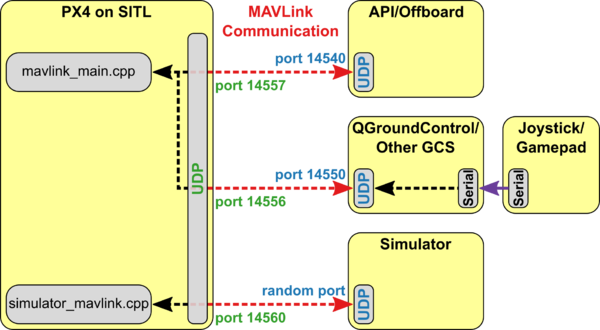
\includegraphics[width=.7\textwidth]{figures/C4/Px4_sitl_overview}
    \caption{SITL with Gazebo architectural scheme}
    \label{fig:SITL-architecture}
\end{figure}

Gazebo offers the possibility to load a satellite map through the \textsf{StaticMap} plugin\footnote{documentation at \url{http://gazebosim.org/tutorials?tut=static_map_plugin&cat=build_world}}. In this way the simulation environment (\autoref{fig:gazebo-Map}) represents \todo{depicts????} quite accurately the real world scenario.
The vehicle used in simulation environment is the 3DR Iris (\autoref{fig:gazebo-iris}), because its model was already created by PX4 team along with different sensors like the 2D 360\degree\ lidar that was used to test object avoidance.
\begin{figure}[ht]
  \centering
  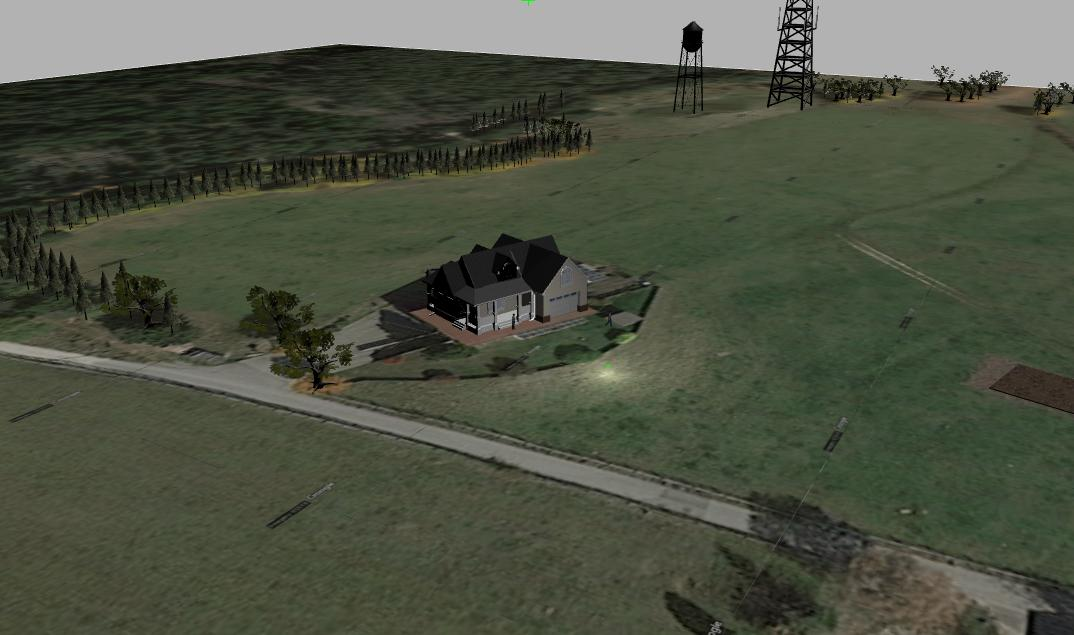
\includegraphics[width=.7\linewidth]{figures/C4/simulation/gazebo-bambi-world.jpg}
  \caption{Gazebo satellite ground plane}
  \label{fig:gazebo-Map}
\end{figure}
\begin{figure}[ht]
  \centering
  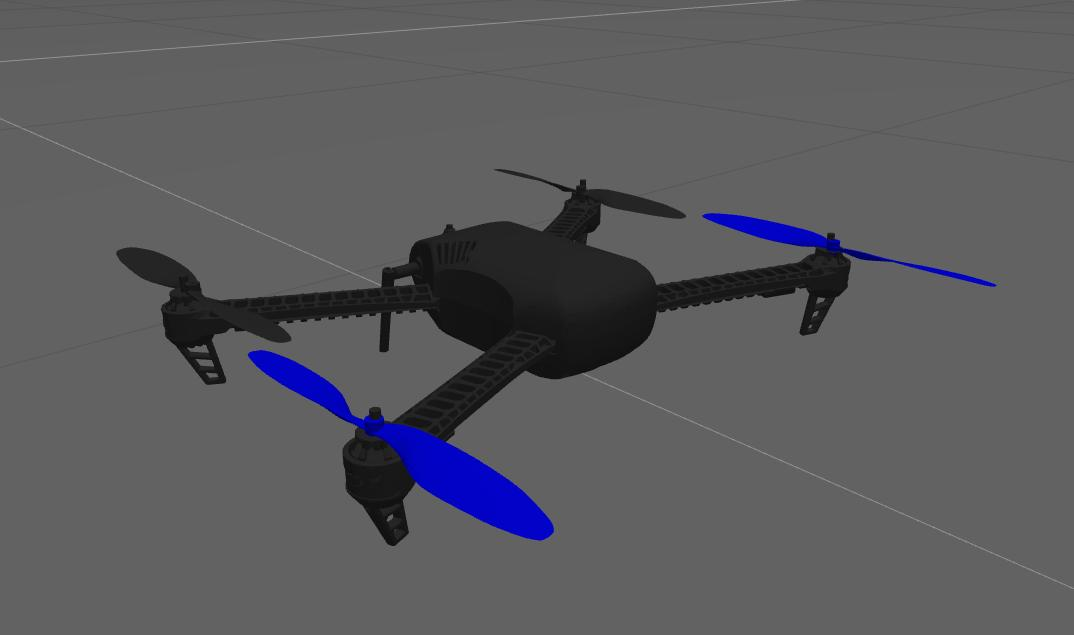
\includegraphics[width=.5\linewidth]{figures/C4/simulation/iris-model1.jpg}
  \caption{Gazebo 3DR iris model}
  \label{fig:gazebo-iris}
\end{figure}
% section simulation_Environment (end)

\section{Starting Bambi Mission} % (fold)
\label{sec:starting_bambi_mission}
Mission start and stop command are issue using the \acrshort{qgc} custom command widget displayed in \autoref{fig:qgc-widget}. This widget was written in \acrfull{qml} an user interface markup language providing an easy way to write simple GUIs \cite{QML}.\\
The button \textsf{BAMBI MISSION START} automatically send the mission start message while \textsf{BAMBI MISSION STOP} send the mission abort message which according to the current mission state causes the \acrshort{uav} to return to the home position or to immediately land at the current position.
\begin{figure}[ht]
  \centering
  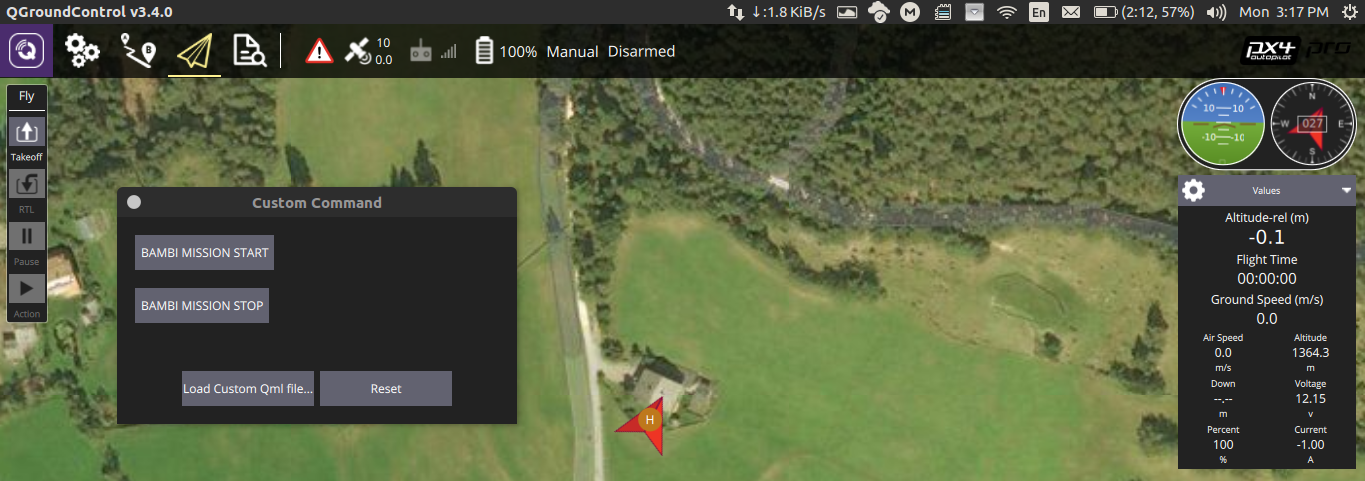
\includegraphics[width=.9\linewidth]{figures/C4/simulation/qgc-widget.png}
  \caption{QGC Bambi's custom command widget}
  \label{fig:qgc-widget}
\end{figure}
% subsection starting_bambi_mission (end)

\section{Testing CPP algorithm} % (fold)
\label{sec:testing_cpp_algorithm}
In order to test the \acrlong{cpp} algorithm it would be necessary to run through the whole mission steps and until the mission controller issue the \textsf{FieldCoverageInfo} message triggering the \acrshort{cpp} node. Therefore to save the time required by the drone to perform the first mission tasks it is convenient to publish a "fake" message directly over the \textsf{/bambi/mission\_controller/trigger\_path\_generation} topic. This is performed executing a simple bash script calling the \textsf{rostopic pub} command.\par
The algorithm was tested using different sample fields. The results obtained for three of them are displayed in \autoref{fig:Coverage-pathGE}. The cellular decomposition consist of $10 \times 10$ cells. \autoref{tbl:fields-area-length} reports the path length compared to the field area which as expected is greater for larger fields.

\begin{table}[ht]
\centering
\begin{tabular}{|l|l|l|}
\hline
\multicolumn{1}{|c|}{\textbf{Field}} & \multicolumn{1}{c|}{\textbf{Area}} & \multicolumn{1}{c|}{\textbf{Path Length}} \\ \hline
1                                    & $15444\, m^2=1.5444\, ha$          & $2.17\, Km$                               \\ \hline
2                                    & $50665\, m^2=5.0665\, ha$          & $5.56\, Km$                               \\ \hline
3                                    & $41586\, m^2=4.1586\, ha$          & $4.66\, Km$                               \\ \hline
\end{tabular}
 \caption{Comparison between field extension and coverage path length}
 \label{tbl:fields-area-length}
\end{table}
\begin{figure}[ht]
	\centering
	\begin{subfigure}{.49\textwidth}
	  \centering
	  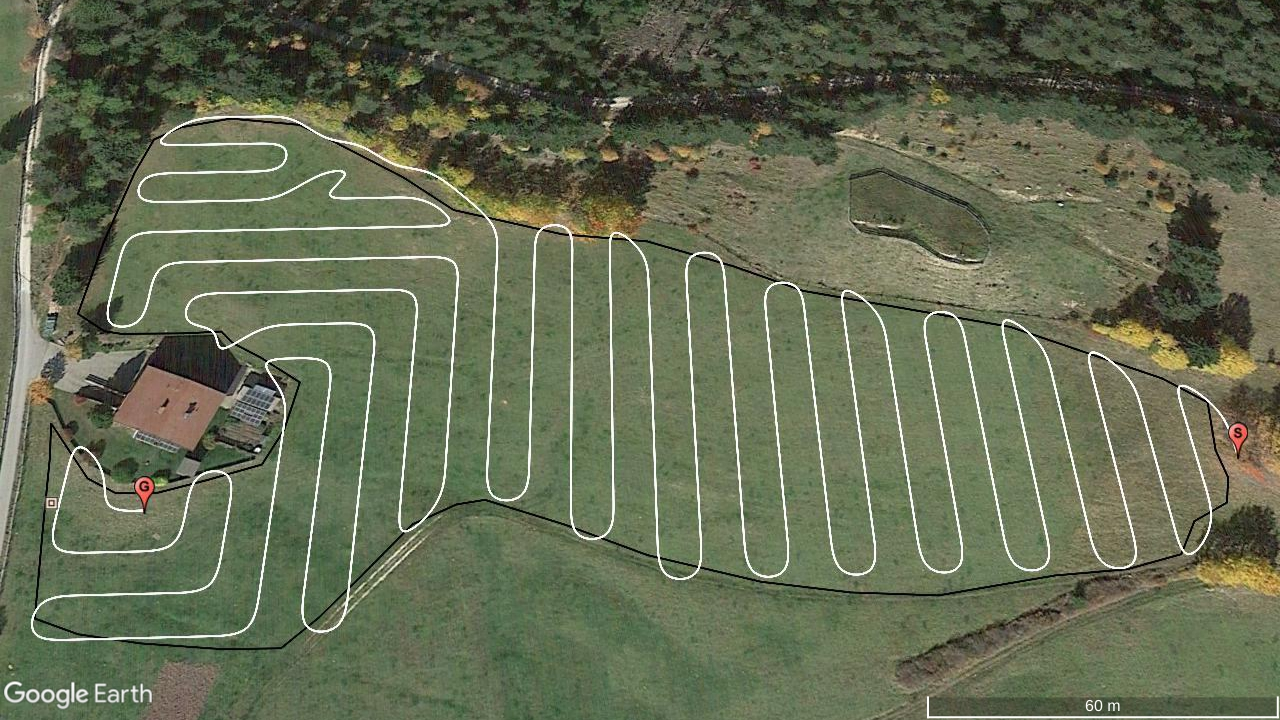
\includegraphics[width=.95\linewidth]{figures/WaldpeterField/Waldpeter-CoverageGE.jpg}
	  \caption{Field 1}
	  \label{sfig:F1-CPP-path}
	\end{subfigure}
	\begin{subfigure}{.5\textwidth}
	  \centering
	  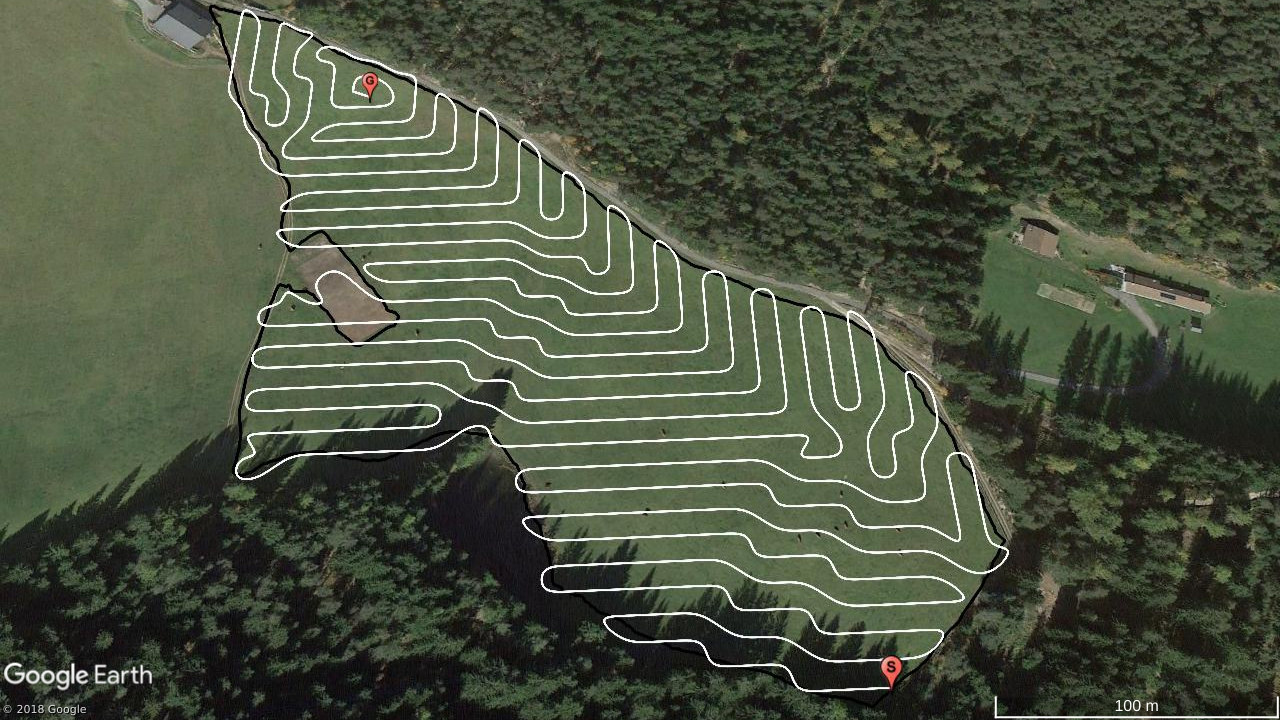
\includegraphics[width=.95\linewidth]{figures/Field2/Field2-CoverageGE.jpg}
	  \caption{Field 2}
	  \label{sfig:F2-CPP-path}
	\end{subfigure}
	\begin{subfigure}{.49\textwidth}
	  \centering
	  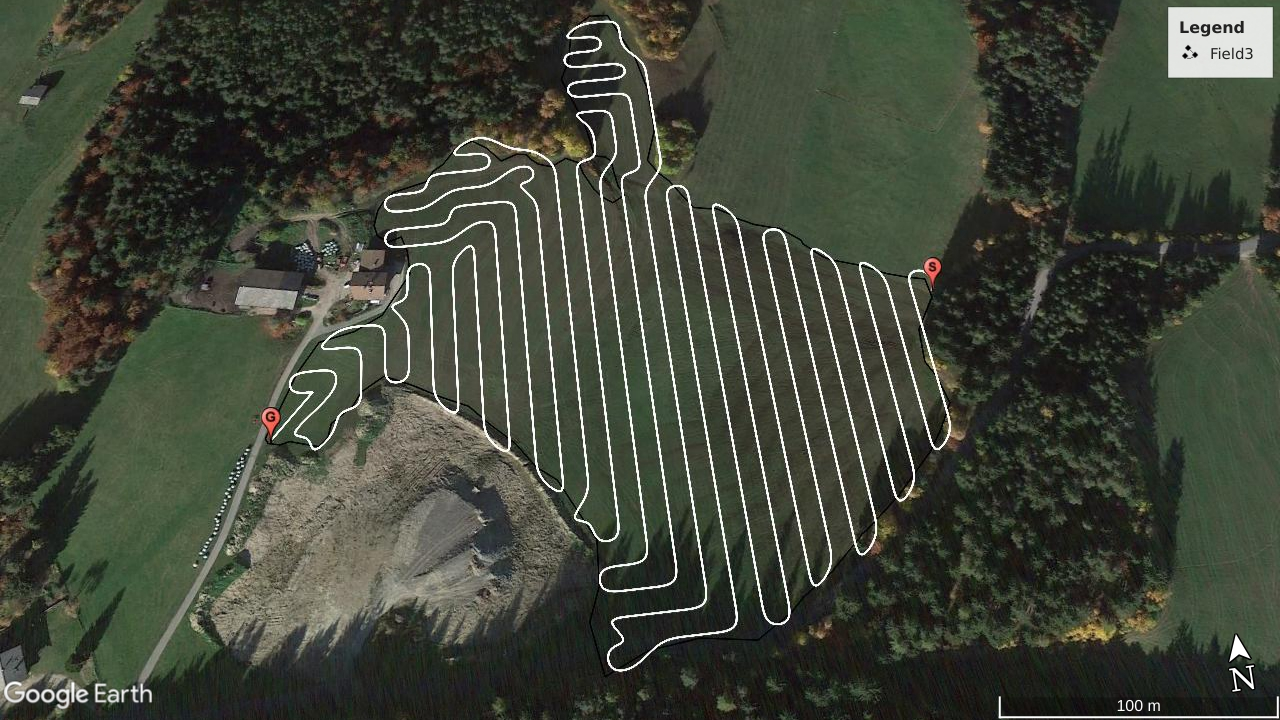
\includegraphics[width=.95\linewidth]{figures/Field3/Field3-CoverageGE.jpg}
	  \caption{Field 3}
	  \label{sfig:F3-CPP-path}
	\end{subfigure}
	\caption{CPP output path applied to different shaped fields}
    \label{fig:Coverage-pathGE}
\end{figure}
% subsection testing_cpp_algorithm (end)

\subsection{Different Starting and Goal Positions} % (fold)
\label{sub:different_starting_and_goal_positions}
During the design of {}the \acrshort{cpp} node several starting and goal position were tested. This helped to understand how the algorithm behaves under different condition and to implement a smart selection of the starting cell. \autoref{fig:coverage-start-goal-pos} shows the outcome path under three different situations.\par
When the starting point is in the middle of the field, as it is in \autoref{sfig:F3-modified-start-pos}, the coverage trajectory starts as a straight line toward the furthest point from the goal position, thought it is the path having the steepest ascending gradient. The cells visited in this transition are marked as visited and therefore avoided in the successive steps. This leads to have such kind of two halves partitioning in the trajectory.\par
The situation radically change if, at the center of the workplace, is placed the goal point. The wave-front propagate all around this position and the generated path assume the spiral like shape in \autoref{sfig:F3-modified-start-goal-pos}. As in the previous situation the path present numerous changes of direction.\par
Finally in \autoref{sfig:F3-regular-start-pos} the starting cell is chosen looking for the farthest most isolated cell with the method presented in \autoref{sub:choosing_starting_position}. The goal position is instead at the extremity of the field and it coincides with the home position, thus the point where the \acrshort{uav} were placed when the mission started. This is reasonable as, in a real situation, where the grass is tall, the mission is suppose to start from the field's border. The resulting path is definitely the best of the three showing a lawnmower like behavior. The prevalence of straight lines limits speed variations, consequently acceleration and power consumption are reduced.
\begin{figure}[ht]
	\centering
	\begin{subfigure}{0.49\textwidth}
	  \centering
	  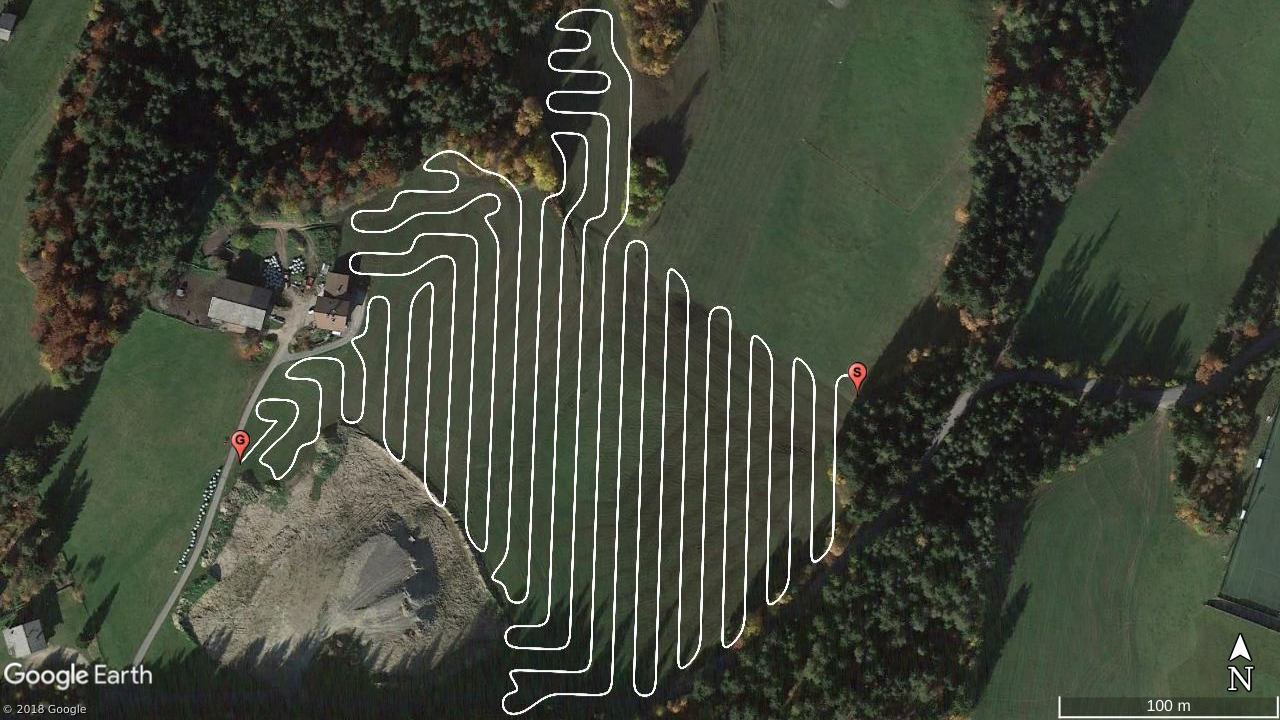
\includegraphics[width=0.95\linewidth]{figures/Field3/Field3-CoverageGE-BSpline-noBorder.jpg}
	  \caption{}
	  \label{sfig:F3-regular-start-pos}
	\end{subfigure}
	\begin{subfigure}{0.49\textwidth}
	  \centering
	  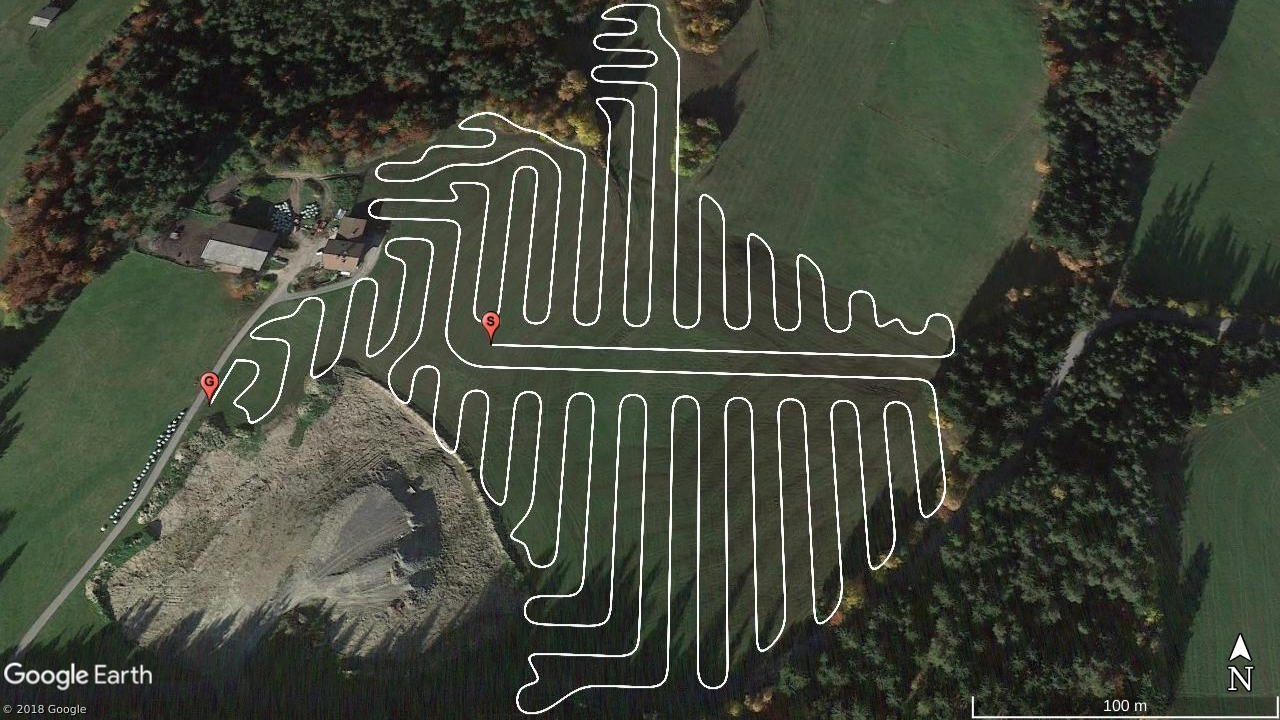
\includegraphics[width=0.95\linewidth]{figures/Field3/Field3-CoverageDifferentStartingPosition.jpg}
	  \caption{}
	  \label{sfig:F3-modified-start-pos}
	\end{subfigure}
	\begin{subfigure}{0.49\textwidth}
	  \centering
	  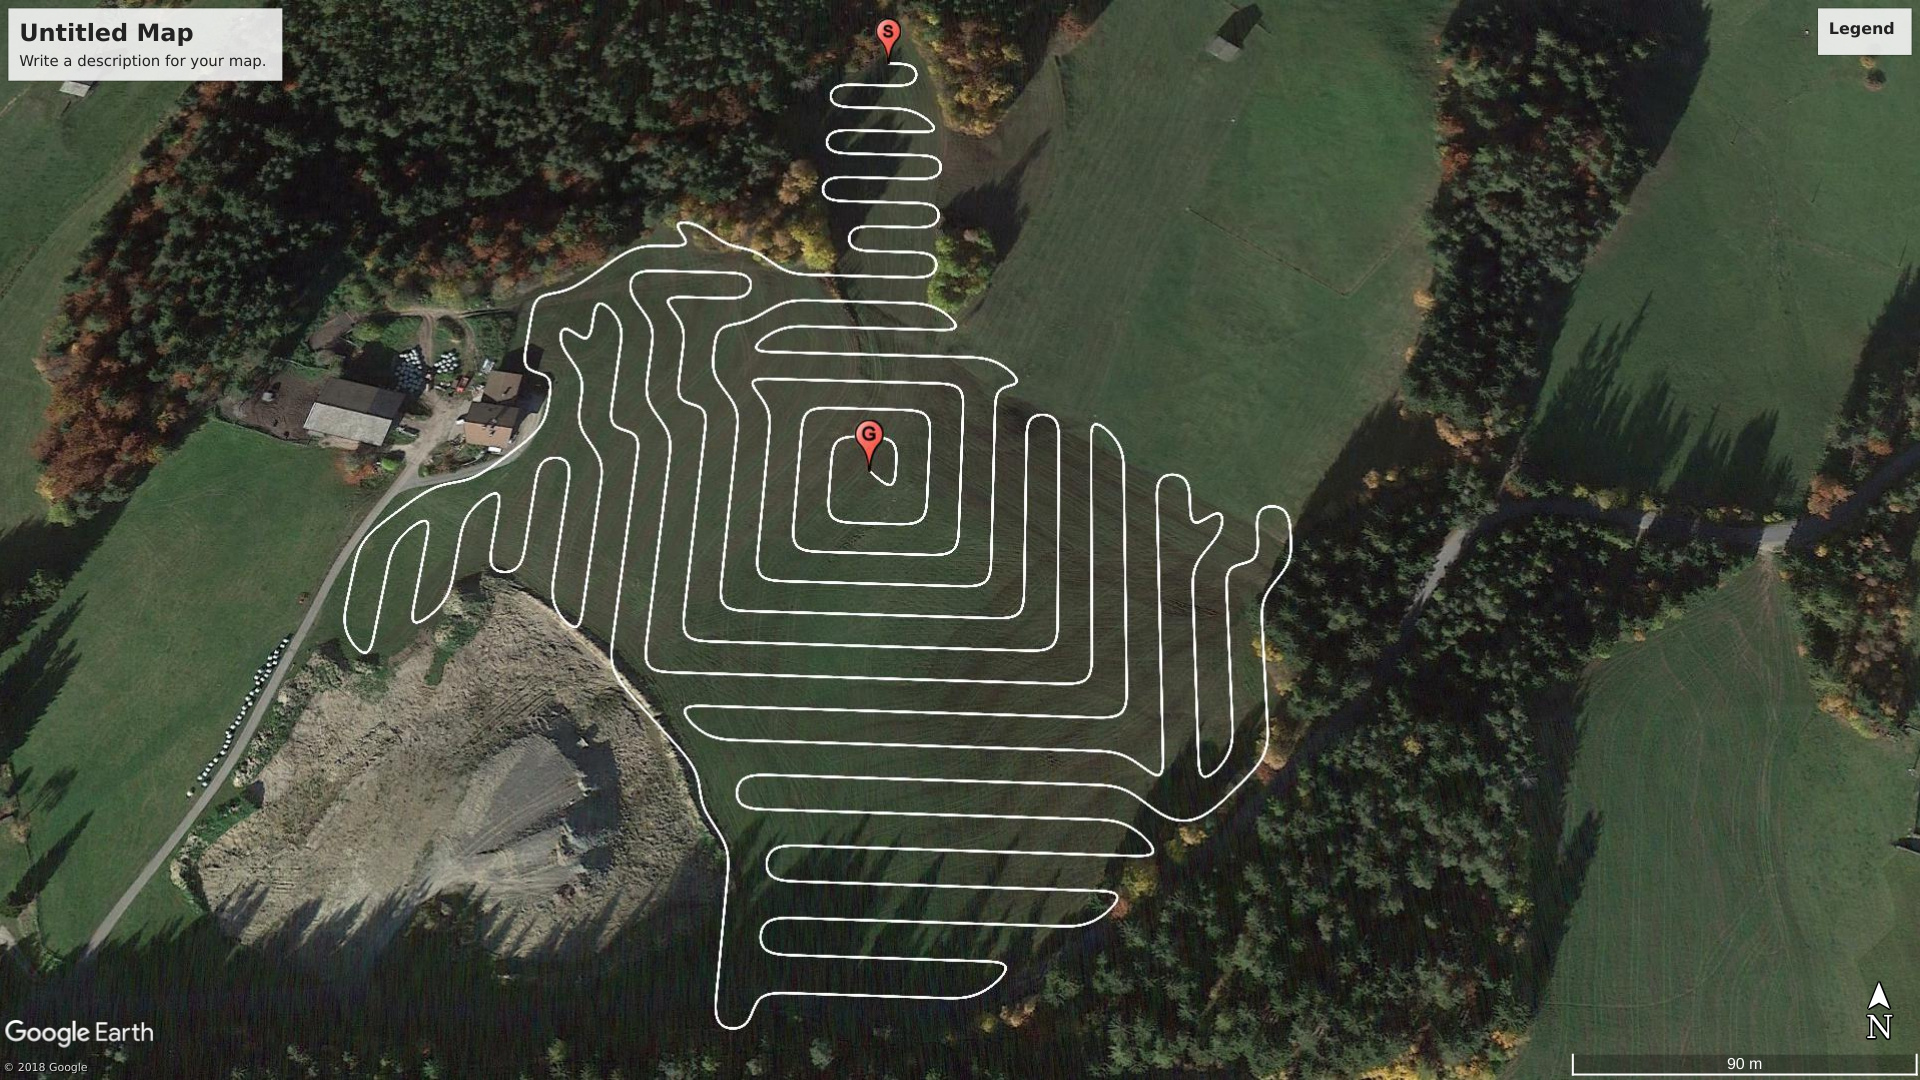
\includegraphics[width=1\linewidth]{figures/Field3/Field3-CoverageDifferentStartingGoalPosition.jpg}
	  \caption{}
	  \label{sfig:F3-modified-start-goal-pos}
	\end{subfigure}
	\caption{Coverage Path generated with Starting and Goal position}
    \label{fig:coverage-start-goal-pos}
\end{figure}
% subsubsection different_starting_and_goal_positions (end)
\subsection{Errors Analysis} % (fold)
\label{sub:errors_analysis}
Looking at the three coverage paths in \autoref{fig:Coverage-pathGE} one can notice that in some section at the border, the trajectory exceed the boundary (represented as black line). This phenomenon is a drawback of the approximate cellular decomposition (see \autoref{sub:approximate_cellular_decomposition}. The algorithm, in fact, marks a cell as part of the field when the intersection between the square polygon of the cell and the field polygon
exist. This cause the cells locate at the edge of the workplace to be marked as field even if just a small portion of them are actually inside the field. This approximation leads to imperfections in the path as shown in \autoref{fig:CPP-imperfections}. The larger are the cells, the greater becomes the effect because the approximation gets worse. For instance using $10 \times 10\, m$ cells the trajectory goes outside the border of a distance as high as $9\, m$.\par
Possible \textit{solutions} could be:
 \begin{enumerate*}
	\item Using a grid with smaller cell,thus increasing the sensor overlap;
	\item Considering a threshold on the intersecting area under which the cell it is no considered as part of the field. This could lead to a not complete coverage of the target area.
	\item In the algorithm handle external cells as particular case and using as waypoint not the center but a point inside the workplace.
\end{enumerate*}

\begin{figure}[ht]
	\centering
	\begin{subfigure}{.49\textwidth}
	  \centering
	  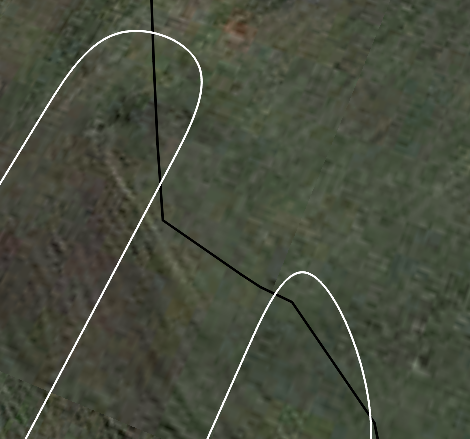
\includegraphics[width=.9\linewidth]{figures/Field3/Field3-imperfection.png}
	  \caption{}
	  \label{sfig:CPP-imperfection1}
	\end{subfigure}
	\begin{subfigure}{.49\textwidth}
	  \centering
	  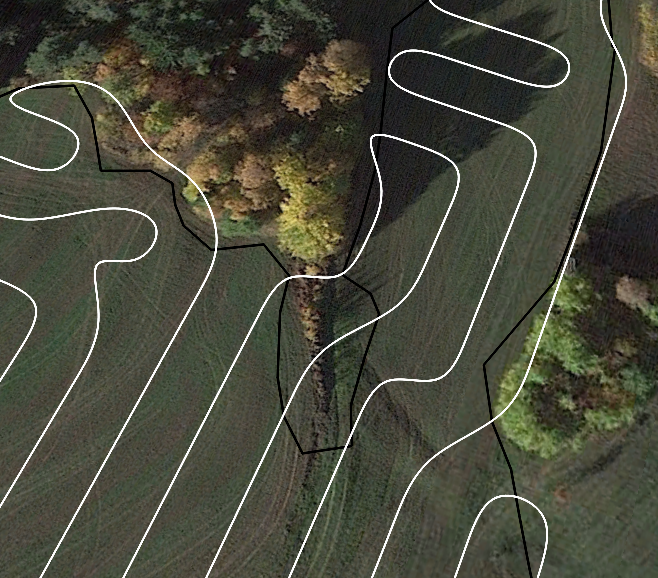
\includegraphics[width=.95\linewidth]{figures/Field3/Field3-imperfection2.png}
	  \caption{}
	  \label{sfig:CPP-imperfection2}
	\end{subfigure}
	\caption{Errors due to Approximate Cellular Decomposition}
    \label{fig:CPP-imperfections}
\end{figure}
% subsubsection errors_analysis (end)
\section{Final Considerations} % (fold)
\label{sec:considerations}
Overall, the generated path (assuming a smart selection of start and goal point) is satisfactory for the desired purpose even if, in some section, there are turns which would be nice to avoid. This is accentuated especially when the workplace has a complex shape (\autoref{sfig:F2-CPP-path}). This shortcoming is something expected, in fact, at the actual development stage only the distance from the goal point is used as cost function in the wave-front propagation algorithm, therefore no optimization for reducing turns has been implemented (see \autoref{sub:wave_front_propagation_algorithm}). The distance transformation used, in fact, leads to a spiral like behavior near the goal cell (discussed in \autoref{ssub:grid_based_methods}), thus it is convenient to set the goal position (home position in the mission) at an extremity of the field. \par
The issue discussed in \autoref{sub:errors_analysis} could cause real problem if at the border of the field there are obstacles risking to make the \acrshort{uav} crash. This, at the actual state of development, is partially addressed relying on the \textit{object avoidance} system that has been implemented inside \textit{PX4 Firmware} which, using potential field, try to push the drone away from surrounding obstacles.\par
Finally, considering that the average flight time of a mid-range drone is between $15$ to $20$ minutes and assuming a flight mean velocity of about $4.5\, m/s$ during the mission duration, the distance it can travel is in the range of $4-5.4\, Km$. This distance is enough to cover a $4\, Ha$ field (\autoref{tbl:fields-area-length}).
% subsubsection considerations (end)


% \textit{Qui mostrero' l'output dell'algoritmo rappresentato come tracciato su google earth. verranno messi a confronto diverse scelte di starting e goal point e discutero' delle performance ottenute con relativi problemi da risolvere}

% \textit{\textbf{Mostrare importanza della scelta della starting position + bezier vs spline interpolation}}
% section simulation_results (end)


















 % Da mettere nel corpo della tesi NON INTRO

% \section{Hardware Setup} % (fold)
% \label{sec:hardware_setup}
% The quadcopter (UAV) is equipped with:
% \begin{itemize}
% 	\item Pixhawk flashed with PX4 flight stack (see appendix \ref{appendix:pixhawk_flight_controller})
% 	\item NEO-M8n (GPS){}
% 	\item 3DR telemetry radio 433Hz (serial link between the UAV and the ground station)
% 	\item LidarLite V3 (altitude distance sensor) \cite{grm:lidarlite}
% 	\item Raspberry Pi 3b (Onboard computer running ROS over Ubuntu OS)
% \end{itemize} 
%  The ground station is composed by a common laptop running QGroundControl \todo{appendix or small description and features of QGC} application. The communication with the UAV uses the MAVLink protocol \cite{Mavlink} through an USB 433Hz telemetry radio .
% % section hardware_setup (end)

% \section{Software} % (fold)
% \label{sec:software}

% \todo{ROS, PX4 why we choose them}
% \todo{ROS design graph and explanation of each node}
% \todo{go deeply in ortho photo a}
% % section software (end)
% section  (end)